\section{Angular JS \textnormal{\textsf{\small{Markus Böbel}}}}

Die Präsentationsschicht des Unternehmensplanspiels besteht wie in Kapitel \ref{sec:architektur} beschrieben aus einer einfachen Webanwendung, einer \acf{SPA}. Dies ist eine Webseite, welche grundlegend nur aus einer einzelnen Seite besteht. Erforderliche Daten werden zur Laufzeit nachgeladen und angezeigt. Somit entsteht eine eigenständige Webanwendung. Für diese Dynamik wird des Öfteren die Webprogrammiersprache JavaScript verwand. Diese ist eine asynchrone Programmiersprache. Der Unterschied zu einer synchronen Sprache zeigt sich im Beispiel einer simplen \acs{HTTP}-Abfrage. Während synchrone Sprachen einen Aufruf starten und bis zum Erhalten der Antwort warten, fahren asynchrone Sprachen fort und realisieren das entgegennehmen durch \texttt{Callbacks}, also Funktionen, welche nachträglich aufgerufen werden, und die Daten übergeben bekommen. Der Vorteil darin besteht, dass die Anwendung flüssiger läuft, da der Programmablauf zu keinem Zeitpunkt gesperrt werden kann. Die schnell wachsende Komplexität des Quellcodes relativiert die genannten Punkte. Im Umkehrschluss würde die Implementierung einer solchen \acl{SPA} sehr komplex und unübersichtlich werden. 

Um dagegen vorzugehen, wurden bestimmte Frameworks entwickelt die Entwickler Möglichkeiten geben, solche Webanwendungen strukturiert und übersichtlich zu entwerfen und implementieren. Eines solcher Frameworks ist Googles AngularJS, welches speziell für die Entwicklung von \acp{SPA} entwickelt wurde. Eine Besonderheit von Angular 2 ist es, dass anstatt reinem JavaScript die Anwendung in TypeScript geschrieben wird.
TypeScript ist eine Erweiterung des ECMA-Script 6 JavaScript Standards und ermöglicht zum einen das Typisieren von Variablen, sowie das Beschreiben von Objekten mit Hilfe von Dekoratoren. (Erkennbar durch ein \texttt{@}- Zeichen) 
Bevor die Webanwendung gestartet werden kann, gilt es das TypeScript wieder in natives JavaScript zu kompilieren.

\subsection{Aufbau einer Angular 2 Anwendung}
Während die erste Version von Angular Webanwendungen durch vereinfachte JavaScript-Skripte entwickelt wurden, ist Angular 2 nun Komponenten-basiert. 
Dies bedeutet, dass die komplette Anwendung in verschiedene Komponenten unterteilt wird, welche eigene Funktionalitäten besitzen. Werden in einem Teil der Webseite zum Beispiel Informationen über ein Unternehmen angezeigt, so wird dies in einem Komponenten beschrieben. In anderen Worten besteht die komplette Anwendung aus ineinander-verschachtelten Komponenten. Neben Komponenten gibt es noch weitere Elemente:

\begin{description}
	\item[Services] Services dienen dazu Daten anzufragen. Angular 2 arbeitet nach dem \ac{MVC}-Pattern, die Services dienen dabei als Model. Sie fragen Daten an und stellen sie den einzelnen Komponenten bereit. Somit werden alle Anfragen an die REST Schnittstelle in Services getätigt. In anderen Worten entsteht eine Verbindung zum Backend nur durch Services.
	\item[Components] Wie oben beschrieben dienen Komponenten dazu die Applikation in viele kleine Teile zu teilen. Sie besitzen ein HTML Template und einen \texttt{Selector}. Der \texttt{Selector} dient dazu den Komponenten anzuzeigen. Dies geschieht über die einfache Erwähnung in einer anderen HTML Seite, beziehungsweise in dem Template eines weiteren Komponenten. Der \texttt{Selector} \texttt{'test-component'} kann somit in anderen HTML Files mit dem Tag \texttt{<test-component></test-component>} eingebunden werden. Zwischen den Tags ist es möglich eine Ladeanzeige zu implementieren. Diese wird solange angezeigt, wie der Komponent geladen wird.
	\item[Modules] Ein Modul ist das oberste Element. In ihm werden alle Elemente wie Komponenten oder Services definiert und integriert. Nur wenn ein Element im entsprechenden Angular-Modul initialisiert wird, kann es verwendet werden. Jedes Modul enthält eine Bootstrapkomponente, welche bei Start des Moduls angezeigt wird.
\end{description}

\begin{figure}[h]
	\centering	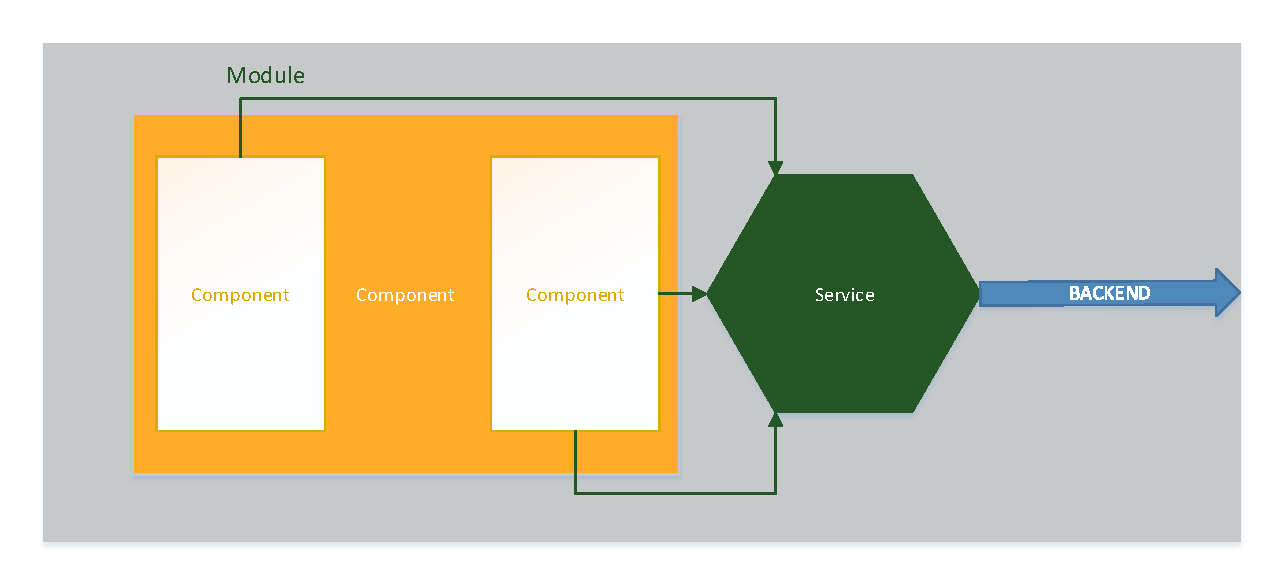
\includegraphics[width=\textwidth]{img/angular2_aufbau}
	\captionsetup{format=hang}
	\caption{
		\label{abb:angular2}Aufbau einer Angular 2 Applikation}
\end{figure}

Im Falle des Fallspieles gibt es 2 Module, welche nebeneinander agieren. Zum einen das \texttt{App}-Modul. Dieses beinhaltet alle Elemente, welche sich um das Login Fenster kümmern. Dazu gehören die entsprechenden Komponenten zur Darstellung der Highscore- oder Spielerliste. Wenn sich der Spieler erfolgreich einloggt gelangt er auf die letztendliche Spielseite. Diese wird strukturiert von \texttt{Home}-Modul. In diesem befinden sich alle Komponenten für die einzelnen Unterseiten.

\subsection{Komponente der Produktion}

Aufgrund der begrenzten Länge der Arbeit wird im Folgenden nur die Komponente der Produktion tiefer erläutert. Diese befindet sich im \texttt{Home}- Modul und wird innerhalb der Home-Komponente angezeigt. 
Der Quelltext \ref{lst:component} zeigt den Grundaufbau einer Komponente. Zuerst wird im obligatorischen \texttt{@Component}-Dekorator der Selector (\texttt{home-component}) angegeben. Ein Zusammenschluss verschiedener Wörter wird dabei über Bindestriche geregelt. Direkt gefolgt davon wird das Template der Komponente angegeben. Dies kann entweder direkt HTML Code sein, oder der Verweis auf eine seperate HTML Datei.
Die letztendliche Komponente wird im Beispiel durch die Klasse \texttt{ProduktionComponent} widergespiegelt. Das Schlüsselwort \texttt{export} ist dabei ein äquivalent zum \texttt{public} in Java. Im Konstruktor der Klasse werden Services übergeben. Diese müssen vorab entweder als Provider im \texttt{@Component}- Dekorator oder im entsprechenden Modul der Komponente angegeben werden.
Im Beispiel der Produktionskomponente \texttt{ProduktionComponent} wird der \texttt{ProduktionService}, welche für die Abteilung der Produktion zuständig ist, sowie der \texttt{HRService}, welcher zum Beispiel für das Einstellen oder Feuern von Personal dient, definiert. Durch das Schlüsselwort \texttt{private} werden die beiden Services als Attribut der Klasse hinterlegt und können von nun an überall in der Komponente verwendet werden.

\lstset{language=Java}
\begin{lstlisting}[float=htbp, caption={Grundaufbau einer Komponente}, label={lst:component}]
	@Component({
		selector   : 'home-component',
		templateUrl: '../../../../templates/components/home.components/produktion.component.html',
	})

	export class ProduktionComponent {
		employees;
		errorMaschinen;
		errorLinie;
		sold;
	
		constructor(private proService:ProduktionService ,private hrService:HRService)
		{
			[...]
		}	
		[...]
	}

\end{lstlisting}

Die Seite der Abteilung Produktion besteht aus mehreren Abschnitten. So soll der Benutzer Lagerhäuser, Produktionsstätten kaufen, sowie seine Maschinen erwerben, verwalten, reparieren und verkaufen können. Des Weiteren soll der Benutzer die Möglichkeit bekommen neue Produktlinien in Produktion zu geben. Diese Funktionen können nun in weitere kleinere Unterkomponenten aufgeteilt werden. So entsteht nun innerhalb der Produktionskomponente folgende neue Unterkomponenten: (siehse Abbildung \ref{abb:productioncomponent})

\begin{figure}[h]
	\centering	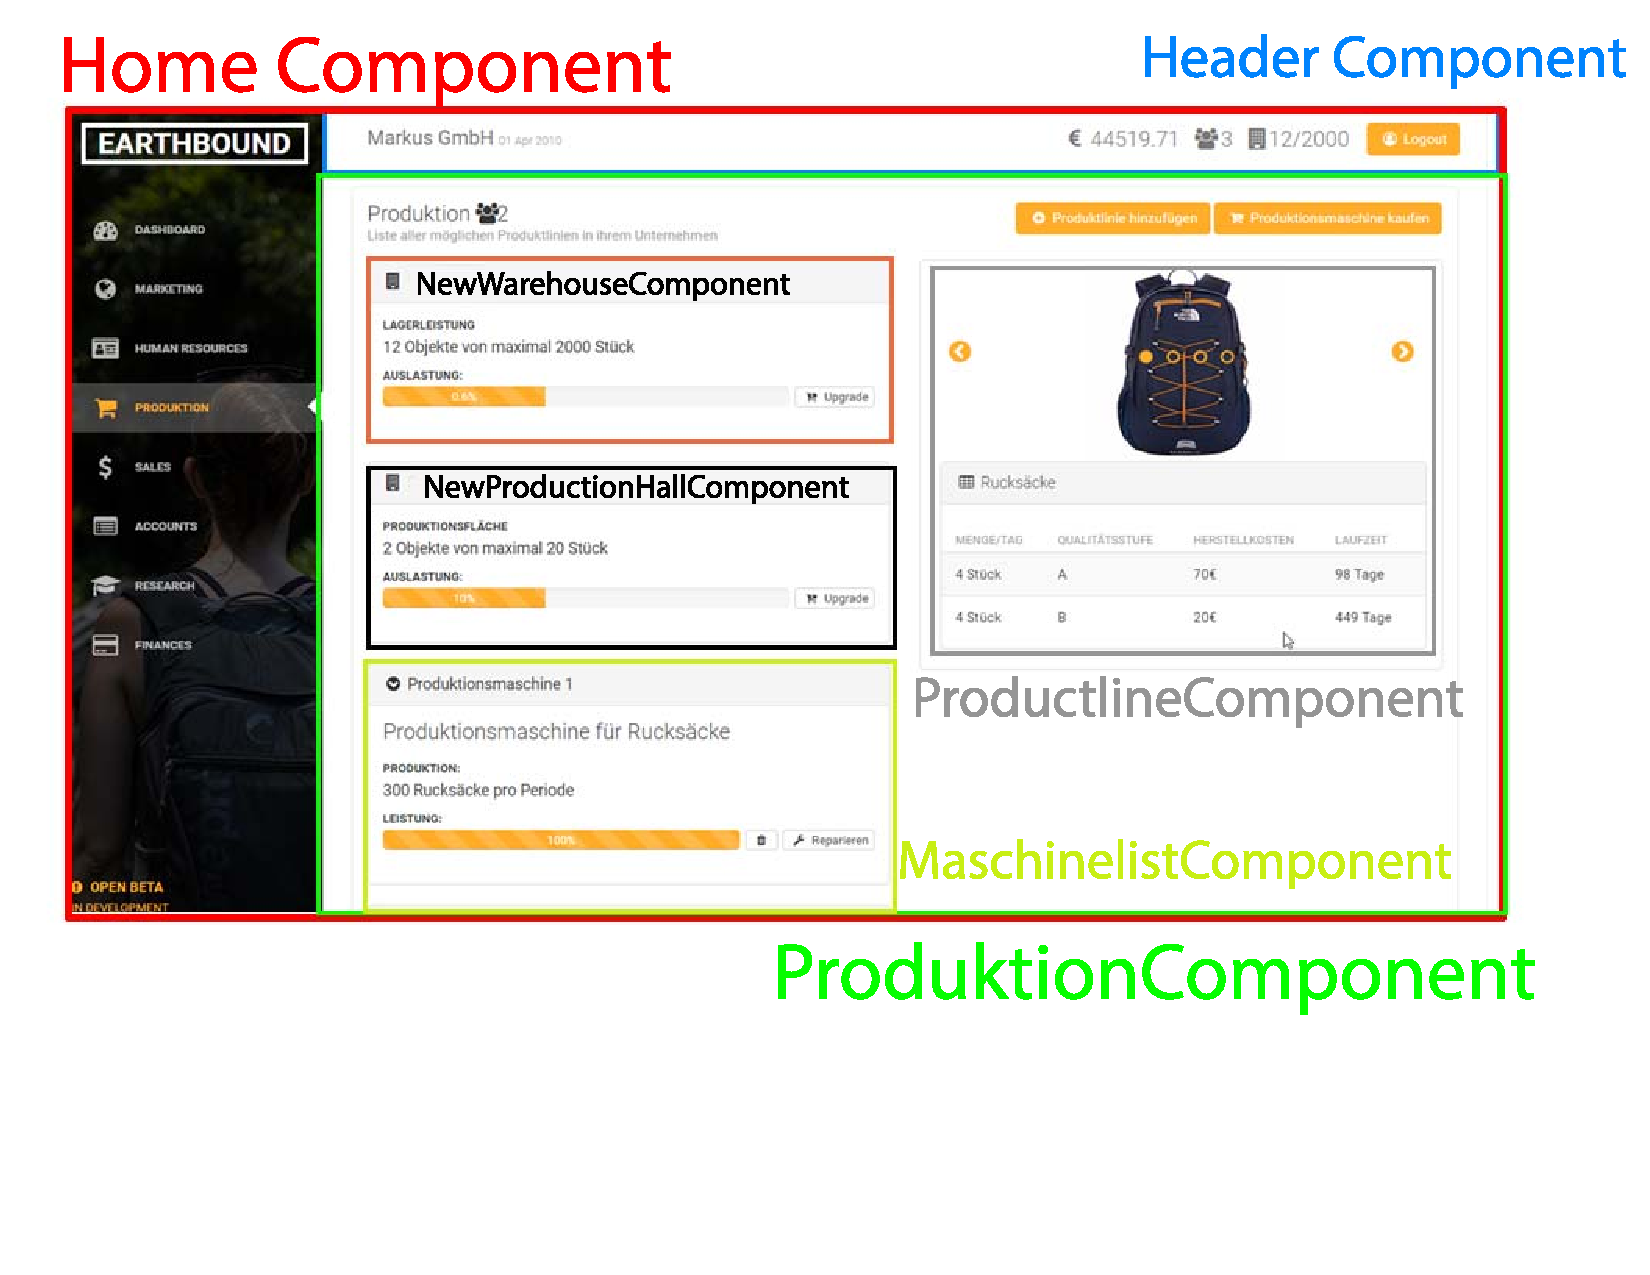
\includegraphics[width=\textwidth]{img/angular2_aufbau2}
	\captionsetup{format=hang}
	\caption{
		\label{abb:productioncomponent}Einteilung der Produktionskomponente }
\end{figure}
\begin{description}
	\item[NewWarehouseComponent] Diese Komponente dient zum Kauf von Lagern und zur Ansicht der Lagerauslastung.
	\item[NewProduktionHallComponent] Diese Komponente ähnelt der des Lagerhauses, dient dennoch zur Verwaltung von Produktionsstätten.
	\item[MachineListComponent] Die Liste der Maschinen wird in dieser Komponente visualisiert. Zudem hat der Spieler zusätzlich die Möglichkeit seine Maschinen zu reparieren oder zu verkaufen. Zudem sieht der Spieler die Abnutzung seiner Maschinen.
	\item[ProductLineListComponent] Diese Komponente dient lediglich zur Visualisierung der aktuellen Produktionen. Dabei hat der Spieler die Möglichkeit zwischen den vier verschiedenen potentiellen Produktionsprodukten hin- und herzuschalten.
	\item[NewProductLineComponent] Auf den ersten Blick versteckt ist die Komponente zur Erstellung neuer Produktlinien. Diese ist ein genanntes Modal, also ein Fenster, welches sich öffnet sofern der Spieler auf den Produktlinie hinzufügen Button auf der oberen rechten Seite der Anwendung klickt.
	\item[NewMachineComponent] Direkt neben dem Button zur Erstellung neuer Produktlinien, befindet sich ein Knopf zum Erwerb neuer Produktionsmaschinen. Dieser öffnet ebenfalls ein solches Modal. 
\end{description}


Die oben beschriebenen Komponenten besitzen einen identischen Grundaufbau verglichen mit dem der Produktionskomponente. Über den angegebenen \texttt{selector} können die Komponenten nun wie oben bereits erwähnt in die Produktionskomponente geladen werden. Die einzelnen Komponente agieren dabei wie ganz normale HTML - Blocktags. (siehe Quelltext \ref{lst:ProduktionHTML})

\lstset{language=HTML}
\begin{lstlisting}[float=htbp, caption={Ausschnitt des Templates  der Produktionskomponente }, label={lst:ProduktionHTML}]
[...]
<div class="content">
	<div class="row">
		<div class="col-md-6">
			<new-warehouse-component>
				Loading
			</new-warehouse-component>
			<new-production-hall-component>
				Loading
			</new-production-hall-component>
			<machine-list-component>
				Loading
			</machine-list-component>
		</div>
		<div class="col-md-6">
			<div class="panel panel-default">
				<productline-list-component>
					Loading
				</productline-list-component>
			</div>
		</div>
	</div>
</div>
[...]
\end{lstlisting}

Wenn nun Daten in die auf dem Interface angezeigt werden, welche als Variable in der Komponente bestehen, dann geht das über die Verwendung geschweifter Klammern. Soll nun zum Beispiel die Variable \texttt{x} ausgeben werden ist dies über \texttt{{{x}}} möglich.
Neben der einfachen Ausgaben unterstützt Angular 2 auch Kontrollstrukturen wie Schleifen (\texttt{*ngFor}) oder Verzweigungen(\texttt{*ngIf}).
Als Beispiel zeigt die Abbildung \ref{lst:MachineList} einen Auszug der Komponente für das Anzeigen und Verwalten von Maschinen.

\lstset{language=HTML}
\begin{lstlisting}[float=htbp, caption={Beispiel für das Anzeigen von Daten in Angular}, label={lst:MachineList}]
   <div *ngFor="let machine of data; let i = index" class="panel-group" id="accordion" role="tablist" aria-multiselectable="true">
	   [...]
			   <p *ngIf="machine.produkt == 'Duffel'">{{machine.kapazitaet}} Duffels pro Periode</p>
		 [...]
	</div>
\end{lstlisting}

Um Daten anzeigen zulassen, müssen diese aus dem Backend geladen werden. Die eigentliche Anfrage findet im Service statt. Dieser stellt nun eine Methode zur Verfügung, mithilfe dessen man die Daten anfragen kann. Als Rückgabewert wird ein sogenanntes \texttt{Observable} zurück gegeben.
Nun kann man dieses \texttt{Observable} abonnieren, das heißt wenn die Anfrage vom Backend beantwortet wird, führt das \texttt{Observable} eine bestimmte Funktion aus. Der Quelltext \ref{lst:DataRequest} der Maschinenlistenkomponente zeigt das Füllen der in Quelltext \ref{lst:MachineList} verwandten Variable \texttt{data}.

\lstset{language=Java}
\begin{lstlisting}[float=htbp, caption={Anfragen von Daten}, label={lst:DataRequest}]
export class MachineListComponent {
	data;

	constructor(private _proService: ProduktionService,[...]) {
		this.loadList();
		[...]
	}
	
	loadList()
	{
		this._proService.getMachines().subscribe(data=>this.data = data);
	}
	[...]
}
\end{lstlisting}

So wird wie im Konstruktor des Komponenten zuerst der Produktionsservice als Attribut der Komponente definiert. Instanzen von Services fangen oftmals mit einem Unterstrich an. Der Konstruktor welcher zu Beginn der Lebenszeit der Komponente aufgerufen wird, führt nun die Methode \texttt{loadList()} aus. Hier wird die Funktion getMachines() des Produktionsservices aufgerufen. Wie zuvor beschrieben gibt diese eine Instanz eines \texttt{Observabels} zurück. Dieses wird nun mit Hilfe der Methode \texttt{subscribe()} abonniert. Als Parameter besteht dabei die Möglichkeit drei Callbackfunktionen anzugeben. Die erste wird ausgeführt, sofern die Anfrage korrekt verlief, die zweite Callbackfunktion dient dazu potentielle Fehler abzufragen. Und als dritten Parameter kann eine Callbackfunktion angegeben werden, welche ausgeführt wird, sofern die Anfrage durchgeführt wurde.
Im Falle des oberen Beispiels, wird bloß eine Funktion angegeben. Diese hat einen Parameter, welche den Rückgabewert der Anfrage enthält, der anschließend in die Variable \texttt{data} der Komponente geschrieben wird. 


Die anderen Komponenten besitzen einen ähnlichen Aufbau und werden aus diesem Grund nicht weiter erläutert. 